%
\documentclass[%
 reprint,
 amsmath,amssymb,
 aps,
]{revtex4-1}

\usepackage{graphicx}% Include figure files
\usepackage{dcolumn}% Align table columns on decimal point
\usepackage{bm}% bold math


\begin{document}



\title{Comparación BD NoSQL}
\author{Yaneth Virginia Aquino Huallpa}
\author{Arlyn Cotrado Coaquira}
\author{Sharon Sosa Bedoya}
\author{Marlon Villegas Arando}
\affiliation{%
 Universidad Privada de Tacna \textbackslash Facultad de Ingenieria \textbackslash Escuela Profesional de Ingenieria de Sistemas
}%


\begin{abstract}
\begin{center}
\textbf{Resumen}
\end{center}

En el presente articulo se relata la comparación hecha de bases de datos NoSQL, describiéndolas y analizando su importancia, así como las definiciones de tipos de bases de datos NoSQL, con el fin de proporcionar un punto de partida para los trabajos en esta área. Y también la creación de una base de datos, inserción y consultas de datos NoSQL mediante Docker.\\

\textbf{Palabras clave:}   NoSQL, Bases de datos, Docker.\\

\begin{center}
\textbf{Abstract}
\end{center}
In the present article the comparison made of NoSQL databases is described, describing them and analyzing their importance, as well as the definitions of NoSQL database types, in order to provide a starting point for work in this area. And also the creation of a database, insertion and queries of NoSQL data through Docker.\\
\textbf{Keywords:}  NoSQL, Databases, Docker.\\

\end{abstract}



\maketitle

%\tableofcontents

\section {Introducción}\label{sec:1}

Dia a día el manejo de la información se hace más complejo; diferentes factores hacen que las personas involucradas en el área busquen tecnologías que le ayuden con este problema. Las bases de datos relacionales son las mas comunes, pero en los últimos años ha aumentado el interés por las bases de datos NoSQL (Not only SQL), un nuevo conjunto de tecnologías que pueden contribuir al manejo de información.
\par Por lo anterior, el presente documento hace una revisión de las tecnologías NoSQL, haciendo posible hacer una comparación.\\

\par El resto de este articulo está organizado de la siguiente manera. En la Sección 2 se muestra los matriales y métodos usados para el desarrollo de este articulo. La Sección 3 se explican los resultados. Y finalmente, las conclusiones están en la Sección 4.



%-----------------------------------------------------------------
\section{Materiales y Métodos}\label{sec:2}
\subsection{Materiales}
	\begin{itemize}
		\item Virtualización activada en el BIOS
		\item Docker Desktop
		\item Windows 10 64bit: Pro, Enterprise o Education, con al menos 4GB de RAM.
	\end{itemize}
\subsection{Métodos}
	\begin{itemize}
		\item Se utilizo como material artículos y libros relacionados a la base de datos NoSQL y sus tipos, así como páginas web.
	\end{itemize}
%-----------------------------------------------------------------
\section{Marco Teórico}\label{sec:3}
\subsection{Base de datos}
	          \begin{itemize}
		\item Una base de datos es una colección de datos organizados según un determinado criterio
		\item Estos datos se pueden leer, crear, actualizar y borrar
		\item También existen motores de base de datos que nos permiten hacer todas estas operaciones de forma más fácil..\cite{Nicolas}
	          \end{itemize}
\subsection{Tipos de base de datos}
	          \begin{itemize}
		\item Existen distintos tipos de bases de datos que se utilizan para solucionar distintos tipos de problemas
                     \item Dentro de la gran familias de bases de datos podemos encontrar las del tipo base de datos relacionales y las no relacionales
		\item Las bases de datos relacionales se conocen generalmente como las SQL
		\item Las no relacionales se conocen como NoSQL
		\item Cada tipo de base de datos tiene beneficios y contras a la hora de almacenar, leer, actualizar o borar los datos
	           \end{itemize}
\subsection{Bases de datos relacional}
	          \begin{itemize}
		\item Desde su definición vemos que una base de datos puede ser relacional si cumple con algo conocido como el modelo relacional.
                     \item En la definición de modelo relacional nos podemos quedar con la idea de tablas que tienen columnas para describir los datos que están relacionados entre si.\cite{comparison}
		\item Ejemplo modelo relacional:\cite{Nicolas}
                     \begin{center}
		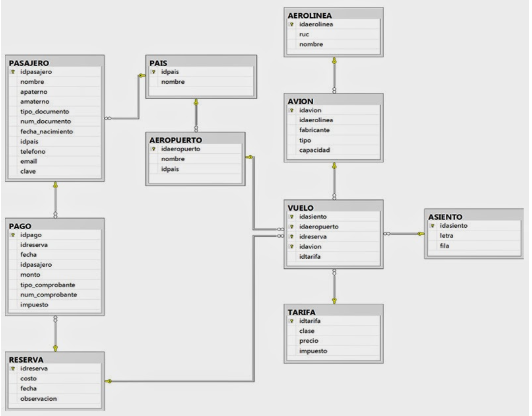
\includegraphics[width=9cm]{./Imagenes/1}
		\end{center}	
	          \end{itemize}
\subsection{Modelo NoSQL}
Este tipo de Base de datos es la respuesta a la necesidad de gestionar volúmenes masivos de información, de tal manera que surge la base de datos NoSQL, término que fue acuñado a finales de los años 90 y que engloba todas las tecnologías de almacenamiento estructurado que no cumplen el esquema relacional, mayormente usado.\\\\
La cantidad de información manejada por las comunidades, redes sociales, buscadores, y muchos otros proyectos en el ámbito de la Web es enorme y abrumadora, lo que ha hecho que surjan nuevas arquitecturas de almacenamiento de información, que deben ser de alto rendimiento, escalables y distribuidas.\\\\
	           \begin{itemize}
		\item Se conoce como NoSQL (Not Only SQL) al grupo de bases de datos que no son relacionales
                     \item Dentro de esta clasificación se encuentran las bases de clave/valor, orientadas a documentos, grafos, de grandes columnas .\cite{Nicolas}
                     \begin{center}
		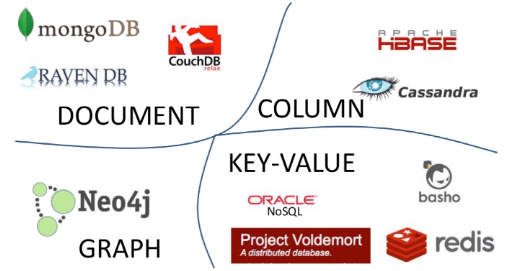
\includegraphics[width=8cm]{./Imagenes/2}
		\end{center}	
		\item Este tipo de bases de datos escala de forma horizontal
		\item Podemos utilizar muchas máquinas chiquitas para crecer y satisfacer las necesidades de los negocios actuales.\cite{Nicolas}
                     \begin{center}
		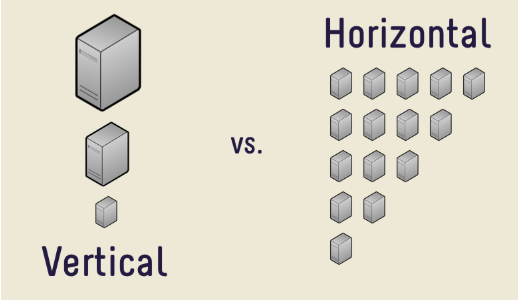
\includegraphics[width=8cm]{./Imagenes/3}
		\end{center}	
	          \end{itemize}
%-----------------------------------------------------------------
\section {Resultados}\label{sec:4}
\subsection{Creacion de base de datos NoSQL con MongoDB}
                     \begin{itemize}
		\item MongoDB es una base NoSQL orientada a documentos
		\item Permite guardar documentos en formato de JSON
		\item Tiene esquema flexible, es decir que podemos cambiar la estructura de nuestros documentos sin ningún problema
                     \item MongoDB está preparado para escalar fácilmente de manera horizontal
                     \item Dado que aprendimos ECMAScript vamos a utilizar un motor de base de datos que nos permite seguir utilizando este lenguaje para guardar nuestros datos.
                     \end{itemize}
\subsection{Instalar MongoDB en Docker}
     \begin{itemize}
                     \item Ingresar sus credenciales creadas en Docker Hub para iniciar sesión en el aplicativo.Ubicar la aplicación PowerShell, ejecutarla como Administrador. En la ventana de comandos de PowerShell escribir lo siguiente.
                     \begin{center}
		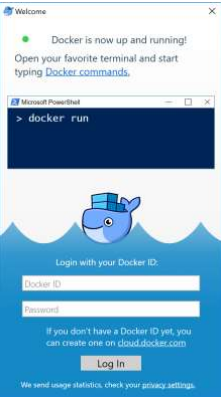
\includegraphics[width=5cm]{./Imagenes/8}
		\end{center}	
		\item Para instalar MongoDB primero tenemos que ejecutar el siguiente codigo.
                     \begin{center}
		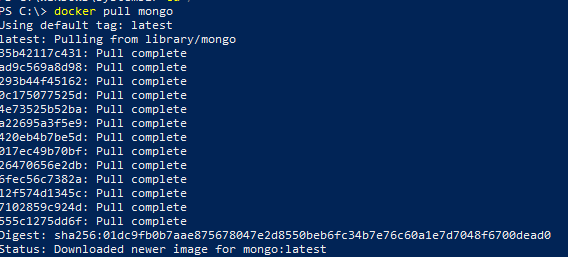
\includegraphics[width=8cm]{./Imagenes/14}
		\end{center}	
		\item Verificar que el contenedor se este ejecutando correctamente mediante el comando:
                     \begin{center}
		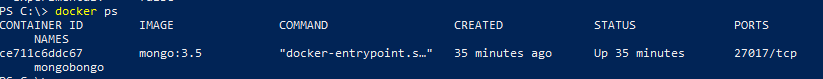
\includegraphics[width=7cm]{./Imagenes/9}
		\end{center}	
                     \item Proceder a verificar la imagen con el siguiente comando:
                     \begin{center}
		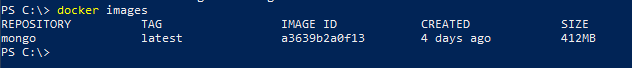
\includegraphics[width=7cm]{./Imagenes/15}
		\end{center}	
                     \item Seguidamente ejecutar el comando.Como respuesta se visualizará un ID que corresponde al contenedor:
                     \begin{center}
		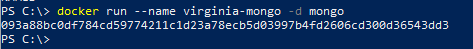
\includegraphics[width=6cm]{./Imagenes/16}
		\end{center}	
                     \item Para conectar  a nuestro localhost 
                     \begin{center}
		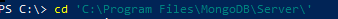
\includegraphics[width=6cm]{./Imagenes/17}
		\end{center}	
                     \item Para exponer ese puerto para nuestro que podamos  acceder al contenedor
                     \begin{center}
		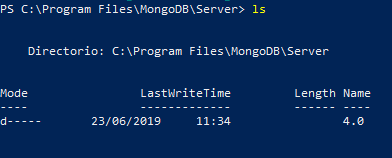
\includegraphics[width=6cm]{./Imagenes/18}
		\end{center}	
                     \item MongoDB está preparado para escalar fácilmente de manera horizontal
                     \begin{center}
		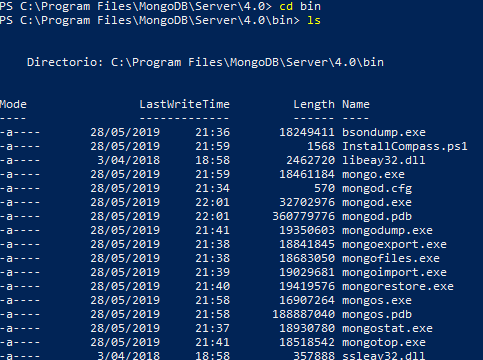
\includegraphics[width=6cm]{./Imagenes/20}
		\end{center}	
                    \item MongoDB está preparado para escalar fácilmente de manera horizontal
                     \begin{center}
		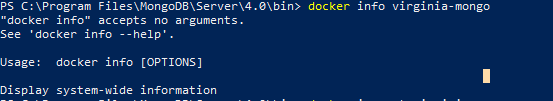
\includegraphics[width=7cm]{./Imagenes/21}
		\end{center}
                     \item MongoDB está preparado para escalar fácilmente de manera horizontal
                     \begin{center}
		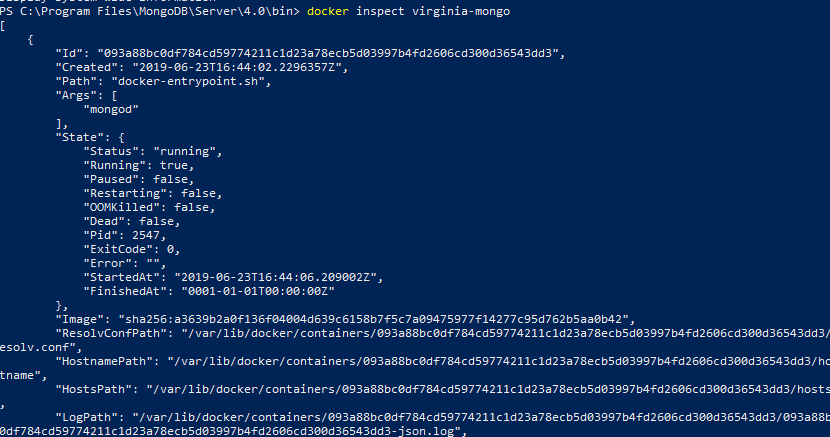
\includegraphics[width=7cm]{./Imagenes/22}
		\end{center}
                     \item En PowerShell ejecutar el siguiente comando ,Verificar la eliminación del contenedor con ejecutando
                     \begin{center}
		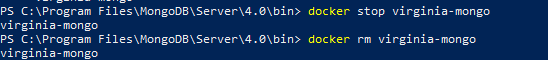
\includegraphics[width=7cm]{./Imagenes/23}
		\end{center}	
                      \item  Seguidamente ejecutar el comando:Como respuesta se visualizará un ID que corresponde al contenedor
                     \begin{center}
		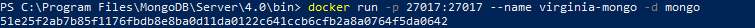
\includegraphics[width=7cm]{./Imagenes/24}
		\end{center}	
                     \item Para conectar  a nuestro localhost 
                     \begin{center}
		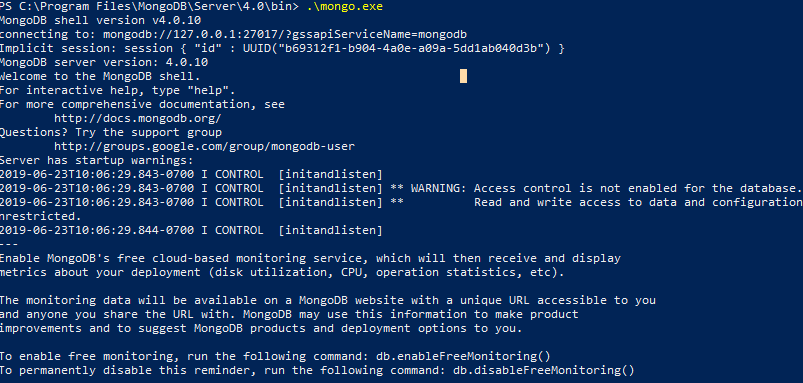
\includegraphics[width=7cm]{./Imagenes/25}
		\end{center}		
	          \end{itemize}
\subsection{Inserción y consulta de datos}
                     \begin{itemize}
		\item conexion de Mongo,instancia de Mongo Corriendo dentro de este contenedor docker 
                      \begin{center}
		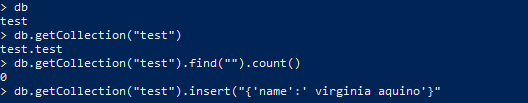
\includegraphics[width=7cm]{./Imagenes/26}
		\end{center}	
		\item Se hace una prueba de Mongo DB,disparar ,para que asi  la base de datos consiga obtener la prueba de recoleccion de datos 
                     \begin{center}
		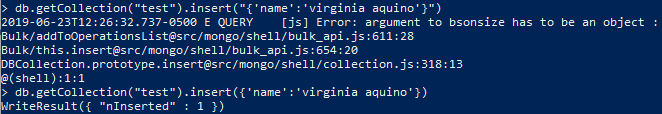
\includegraphics[width=7cm]{./Imagenes/27}
		\end{center}	
                  
	          \end{itemize}
\subsection{Comparación}
\subsection{Documental}
 La popularidad del término "base de datos orientada a documentos" o "almacén de documentos" ha crecido a la par con el uso del término NoSQL.\\
\\ Una base de datos NoSQL documental sirve para gestionar información orientada a documentos o datos semi-estructurados, que se almacenarán en forma de documento.\cite{tesis}
\\\\Normalmente los documentos se estructuran dentro de una serie de contenedores llamadas colecciones (en inglés “collections”) que son proporcionados por el sistema gestor documental. Estas utilizan punteros para el acceso de la información almacenada en la base de datos, esto se realiza sin la ayuda de una estructura entidad relación predeterminada, como en el caso de las bases de datos relacionales.\\
La búsqueda de la información se realiza con base al contenido del documento. \\\\
Las codificaciones más habituales de estos documentos suelen ser XML, YAML o JSON, pero también se pueden almacenar en formato Word o PDF. \cite{proyecto} Las bases de datos de tipo documental son una forma moderna de almacenar datos en formato JSON en lugar de filas y columnas como en las bases de datos relacionales; y esto permite expresar los datos en su forma natural. \\\\
\begin{center}
	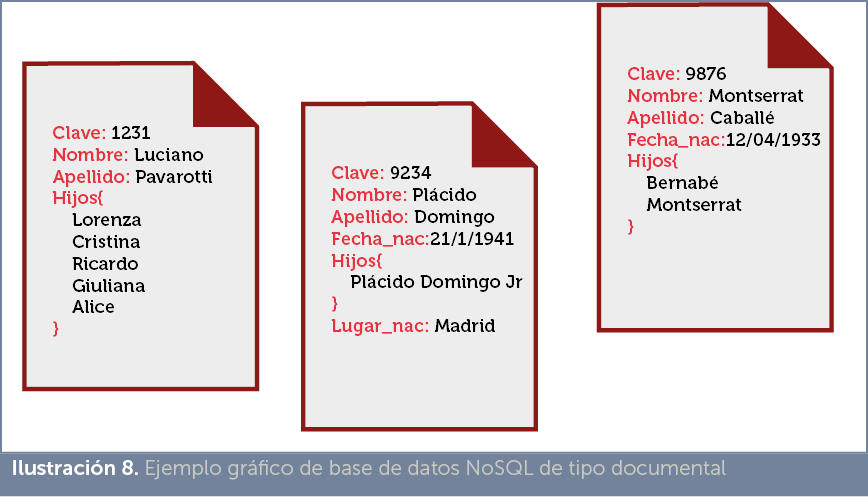
\includegraphics[width=8cm]{./Imagenes/documental1}
\end{center}	
.\\
\textbf{Fundamentos del formato JSON :}
\begin{itemize}
		\item Pares de valores clave o atributos :  Con el formato JSON se almacena en un par de valores clave. A estos pares se les llama a veces atributos. Las claves son cadenas simples y los valores pueden ser de cualquier tipo.\cite{kyocera}
		\item Incrustación de objetos: Los valores incluidos en el par de valores clave también pueden ser otros objetos JSON, lo que permite crear una jerarquía de objetos. Colocar objetos JSON dentro de otro objeto JSON se denomina modelo de datos incrustados en base de datos documentales.\cite{kyocera}
		\item Matrices: El formato JSON trabaja con un lenguaje de programación natural en todos los lenguajes de programación y estructuras de datos que son las matrices, por lo cual se admite almacenamiento de matrices como valores contra una clave. \cite{kyocera}
\end{itemize}
\begin{center}
	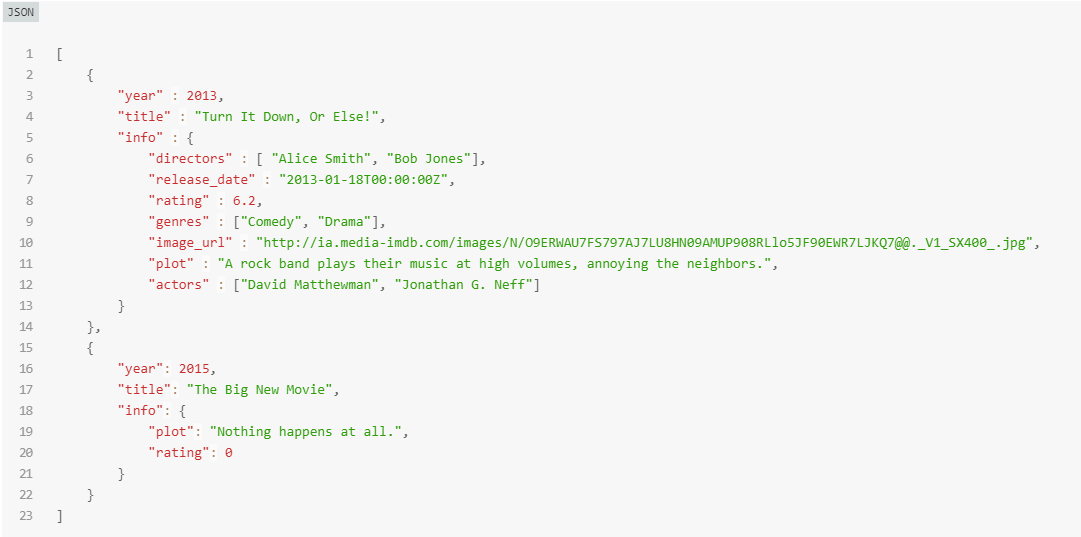
\includegraphics[width=9cm]{./Imagenes/documental2}
\end{center}	
En la imagen podemos ver un ejemplo de un documento de tipo JSON describe un libro.\cite{imagen}\\\\
\textbf{ Factores que influyen en la aceptación de una BD NoSQL documental :}
\begin{itemize}
		\item Adopción de un nuevo paradigma: Este factor de adaptarse al concepto de NoSQL, resulta ser relativamente difícil, ya que la gran mayoría de compañías se encuentran más familiarizadas con las bases de datos relacionales.
		\item Curva de aprendizaje: al ser una tecnología relativamente nueva, esto representa para algunas personas un obstáculo en aprender la utilización de las bases de datos NoSQL
		\item Costo-beneficio: es uno de los factores más importantes, debido al hecho de comparar si los beneficios que se obtendrán son mayores a los costos de implementarlo.                     
\end{itemize}
\textbf{Bases de Datos Documental más conocidas :}
\begin{itemize}
		\item Amazon DocumentDB (compatible con MongoDB): Servicio de base de datos de documentos rápido, escalable, de alta disponibilidad y completamente administrado que es compatible con cargas de trabajo de MongoDB.
		\item MongoDB : Base de datos no relacional de código abierto que ofrece soporte para sistemas de almacenamiento de estilo JSON orientados a documentos.
		\item Couchbase : Plataforma de datos de clase empresarial Couchbase incluye Couchbase Server y Couchbase Mobile, y ha sido diseñada para aprovechar toda la potencia de las aplicaciones móviles, IoT y web. 
		\item RavenDB:  Base de datos orientada a documentos de código abierto escrito en .NET, ofrece un modelo de datos flexible, diseñado para hacer frente a los requerimientos provenientes de los sistemas.                     
\end{itemize}
\subsection{Clave-Valor}
Las bases de datos clave – valor, llamadas tablas también, se estructuran almacenando la información como si de un diccionario se tratara. \\\\ 
Esta moderna forma de almacenamiento clave – valor se caracterizan por tener una elevada escalabilidad y un rendimiento muy bueno para volúmenes de datos muy grandes,  a cambio de ser muy simples y renunciar a funcionalidades que tenemos en otros sistemas como la verificación intrínseca de la integridad de datos, llaves extranjeras y disparadores. \\\\
En las BD de clave valor existen los“contenedores”, y dentro de ellos se pueden almacenar tantos pares clave-valor como se desee. \\\\ Las validaciones de los datos se delegan completamente en la aplicación cliente, siendo la base de datos, simplemente el lugar donde se guardan los datos. No se verifican integridades, no se comprueban referencias cruzadas, todo esto se ha de implementar a nivel de aplicación, en el código del cliente.\\\\
\textbf{Características :}
\begin{itemize}
		\item Una base de datos clave-valor almacena datos como un conjunto de pares clave-valor en los que una clave sirve como un identificador único.
		\item  Tanto las claves como los valores pueden ser cualquier cosa, desde objetos simples hasta objetos compuestos complejos. 
		\item Las bases de datos clave-valor son altamente divisibles.
		\item Permiten el escalado horizontal a escalas que otros tipos de bases de datos no pueden alcanzar.                
\end{itemize}
  \begin{center}
	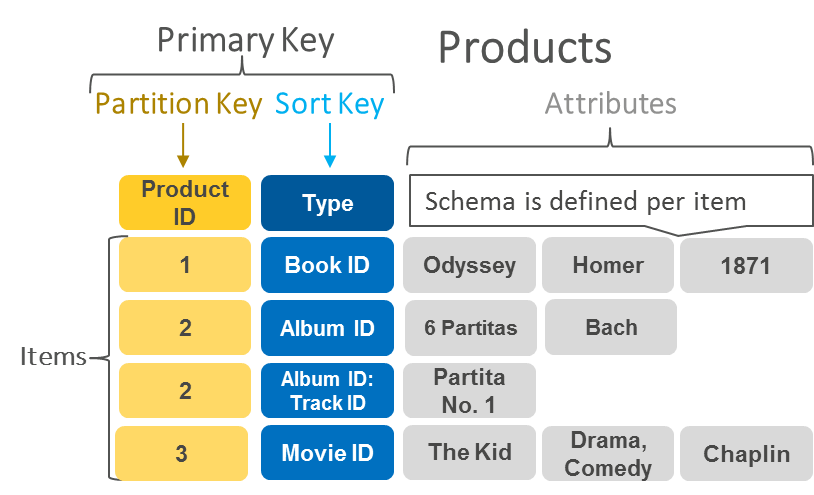
\includegraphics[width=8cm]{./Imagenes/clave1}
\end{center}	
En la imagen podemos ver un diagrama de datos almacenados como pares clave-valor en DynamoDB.\cite{imagen2}\\\\
\textbf{Bases de Datos de Clave-Valor más conocidas :}
\begin{itemize}
		\item DynamoDB : El servicio de Amazon permite únicamente crear nuevas tablas en las que alojar los datos, e interactuar con ellas mediante tus aplicaciones a través de APIs.
		\item Redis : Base de datos en memoria de conjuntos clave – valor, que además permite persistir los datos que residen en memoria a disco.
		\item Apache Cassandra : Base de datos no relacional de alto rendimiento utilizada comúnmente.
		\item RavenDB:  Base de datos orientada a documentos de código abierto escrito en .NET, ofrece un modelo de datos flexible, diseñado para hacer frente a los requerimientos provenientes de los sistemas.                     
\end{itemize}
Los almacenes de llaves valor son útiles para operaciones sencillas, que se basan solo en los atributos clave. Su objetivo es facilitar el acceso a datos.\\\\
\subsection{Grafos}
\begin{itemize}
		\item Estas bases de datos utilizan el modelo de Grafos
		\item Se especializan en relaciones
		\item Las podemos utilizar por ejemplo para guardar puntos de un camino, relaciones de amigos, familia, o cualquier tipo de  dato que represente alguna relación
                     \item Entre los motores más conocidos de este tipo se encuentra Neo4j
                     \begin{center}
		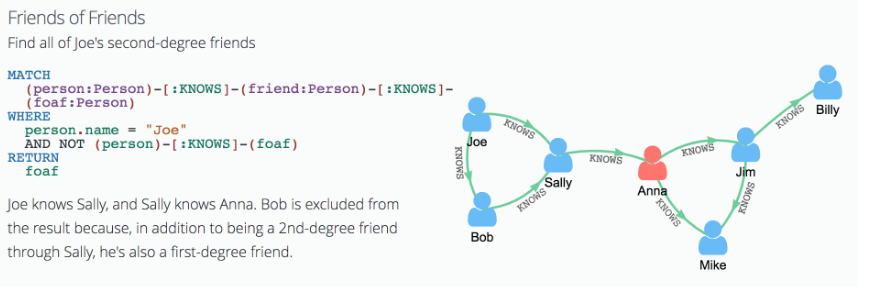
\includegraphics[width=8cm]{./Imagenes/4}
		\end{center}	
	          \end{itemize}
.
\subsection{Tabular (Column-Store)}
\begin{itemize}
		\item Este tipo de familia de bases de datos está orientada a grandes cantidades de datos.
		\item Lo datos son almacenados en columnas.
		\item En una columna tiene múltiples datos.
                     \item Entre los motores más conocidos de este tipo se encuentra Cassandra o HBase.
	          \end{itemize} 
 \begin{center}
	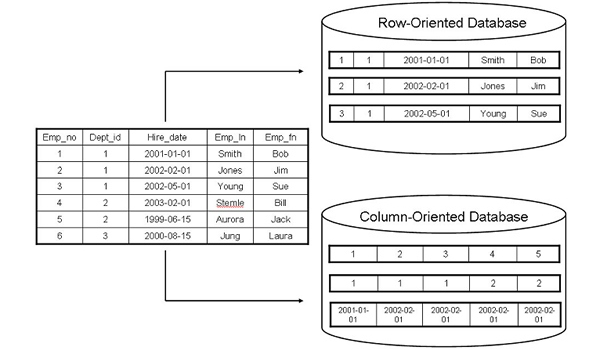
\includegraphics[width=9cm]{./Imagenes/5}
\end{center}	
\subsection{Comparación entre BD Documental y Clave-Valor}
		\begin{center}
		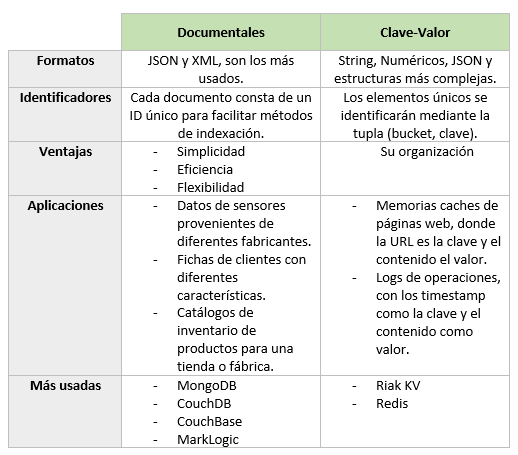
\includegraphics[width=10cm,height=9cm]{./Imagenes/cuadro}
		\end{center}	
%-----------------------------------------------------------------
\section{Discusión y Conclusiones}\label{sec:5}
	\begin{itemize}
		\item NoSQL permite el manejo de grandes volúmenes de datos y la posibilidad de tener un sistema distribuido.
		\item Las características de las bases de datos NoSQL responden a las necesidades actuales de las diferentes organizaciones, por lo que son una alternativa debido a su capacidad y a la velocidad.
		\item La integración de ambos, NoSQL y bases de datos relacionales, es un área que debería ser explorada. Las base de datos NoSQL comercializa funciones de confiabilidad y consistencia para un rendimiento y proceso de escalabilidad extremo, convirtiendolo en una solución especializada, ya que el número de aplicaciones que pueden depender de las bases de datos NoSQL sigue siendo limitado.
	\end{itemize}


% Bibliografia.
%-----------------------------------------------------------------

\bibliographystyle{plain}
\bibliography{Bibliografia}

\end{document}
